\chapter{Statistiques descriptives du jeu de données}
\section*{Division du dataset}
Le jeu de données a été divisé en trois parties : entraînement, validation et test. Voici la répartition du nombre de commentaires dans chacune de ces parties :
\begin{table}[h]
\centering
\begin{tabular}{lc}
\toprule
\textbf{Catégorie} & \textbf{Nombre de commentaires} \\
\midrule
Train & 127,656 \\
Validation & 31,915 \\
Test & 63,978 \\
\bottomrule
\end{tabular}
\caption{Répartition du nombre de commentaires}
\end{table}


\section*{Répartition des labels}
Les commentaires toxiques sont minoritaires dans l'ensemble de données. 
En effet, il y a \textbf{10.2\%} de commentaire globalement non toxiques. 
Cela peut poser des problèmes lors de l'entraînement des modèles, car les classes minoritaires peuvent être sous-représentées et donc mal apprises.
La répartition des labels de toxicité est également inégale.
La somme des pourcentages n'est pas égale à 100\% car un commentaire peut avoir plusieurs labels. 
C'est donc un problème de classification \textit{multi labels}.
\begin{table}[h]
\centering
\begin{tabular}{lc}
\toprule
\textbf{Label} & \textbf{Pourcentage} \\
\midrule
toxic & 94.3\% \\
severe\_toxic & 9.8\% \\
obscene & 51.9\% \\
threat & 3.1\% \\
insult & 48.2\% \\
identity-hate & 8.6\% \\ % Replace X.X with the actual value
\bottomrule
\end{tabular}
\caption{Répartition des labels sur les commentaires globalement toxiques}
\end{table}


\newpage
\section*{Corrélation entre les labels}
Les labels de toxicité présentent une forte corrélation entre eux. 
Il est possible d'anticiper dès à présent une difficulté du modèle à distinguer un commentaire toxique d'un commentaire obscène (\textbf{74\%} de corrélation).
Cela représente un point à prendre en compte lors de la conception du modèle. La matrice de corrélation est incluse dans l'annexe \ref{chap:appendix}. 

\section*{Longueur des commentaires}
La distribution de la longueur des commentaires est très variée. En effet, l'écart-type est bien plus élevé que la moyenne. 
La longueur moyenne des commentaires est de \textbf{395} caractères, avec un écart-type de \textbf{593} caractères. 
Cela peut poser des défis lors de la conception du modèle. Il est crucial de prétraiter les données pour normaliser la longueur des commentaires.
\begin{figure}[h]
    \centering
    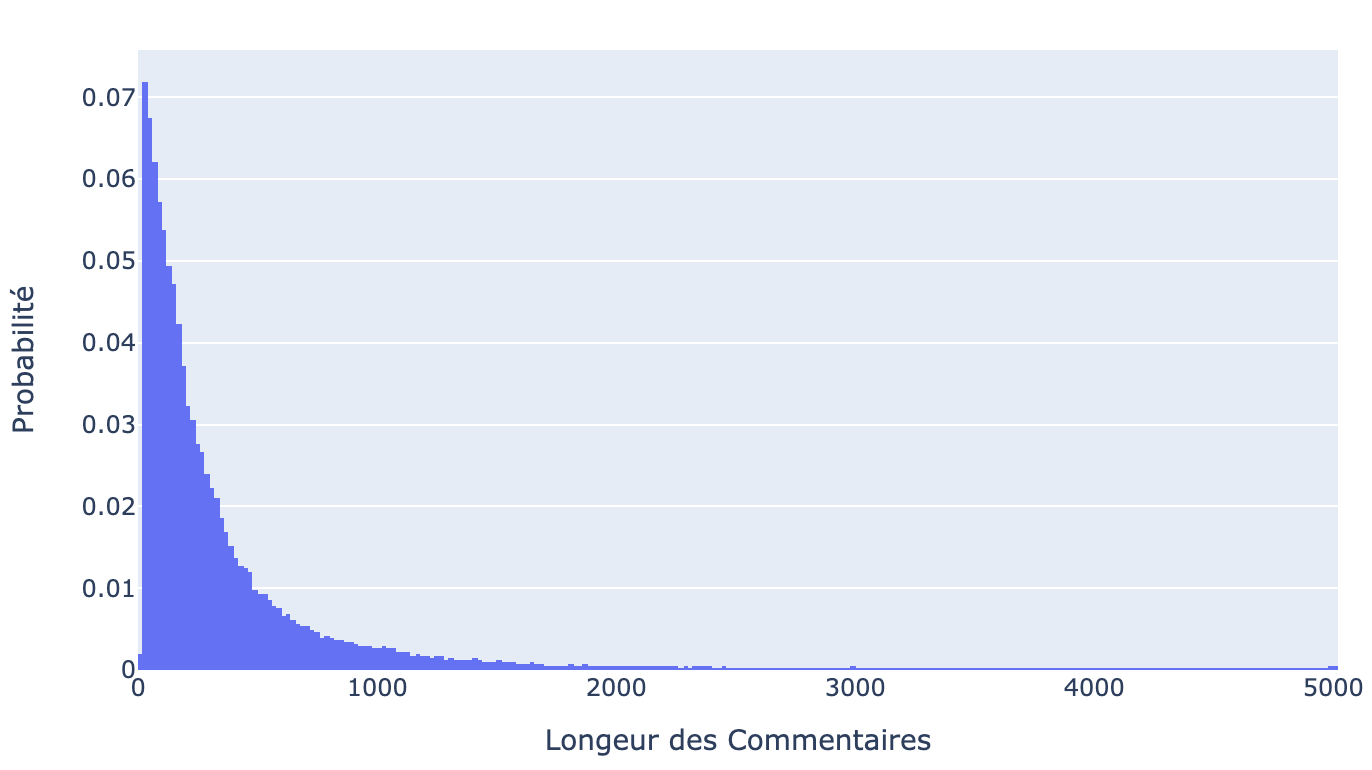
\includegraphics[width=0.5\textwidth]{figures/long-commentaire-prob.png}
    \caption{Distribution de la longueur des commentaires}
\end{figure}

\section*{Distribution des mots}
Dans le jeu de données, environ \textbf{180 000} mots uniques sont recensés. 
Sans surprise, les mots les plus fréquents sont les mots de liaison et les mots vides.
Cependant, en raison de la source du jeu de données, les termes \textbf{articles}, \textbf{wikipedia} et \textbf{pages} apparaissent également très souvent dans les commentaires (respectivement en 26e, 30e et 31e positions).
En effet, les utilisateurs citent souvent des sources pour appuyer leurs propos. Dans les commentaires toxiques, des insultes, des mots vulgaires et des termes discriminatoires sont fréquemment observés. 
La visualisation de ces derniers à l'aide de \textit{WordCloud} permet de représenter visuellement les mots les plus utilisés. 
En annexe \ref{chap:appendix}, une représentation \textit{WordCloud} des commentaires du jeu de données, filtrée selon le type de toxicité est présentée.